\documentclass[10pt,a4paper]{article}
\usepackage[utf8]{inputenc}
\usepackage{amsmath}
\usepackage{amsfonts}
\usepackage{amssymb}
\usepackage[left=2cm,right=2cm,top=2cm,bottom=2cm]{geometry}
\usepackage{parskip}
\DeclareMathOperator*{\argmin}{arg\,min}
\usepackage{float}
\usepackage{tikz}
\author{Garrick Lin}
\title{Convex Optimization Note}
\begin{document}
\maketitle

\section{Affine Set}

\subsection{Definition}
A set $\mathcal{A}$ is called affine set when it satisfied:
\begin{quotation}
	If $\mathbf{x_{1}} \in \mathcal{A}$ and $\mathbf{x_{2}} \in \mathcal{A}$, then, $\forall \theta \in \mathcal{R}$, $x = \theta \mathbf{x_{1}} + (1 - \theta) \mathbf{x_{2}}$ also belong to $\mathcal{A}$. 
\end{quotation}
The expression $\theta \mathbf{x_{1}} + (1 - \theta) \mathbf{x_{2}}$ represent a line that cross through $\mathbf{x_{1}}$ and $\mathbf{x_{2}}$. Hence, affine set can be explained intuitively as:
\begin{quote}
	Affine set is a set that contain the line which cross through any two point within this set.
\end{quote} 

\subsection{Properties}
Assume a affine set $\mathcal{A} \subseteq \mathcal{R}^{n}$. If $\mathcal{A}$ contain original point($\mathbf{0}$), then, $\mathcal{A}$ is a subspace. In order to prove this, $\mathcal{A}$ must satisfied following three rules:  
\begin{enumerate}
	\item $\mathcal{A}$ contain original point.
	\item If $\mathbf{v} \in \mathcal{A}$, then, $\forall \theta \in \mathcal{R}$, $\theta \mathbf{v} \in \mathcal{A}$.
	\item If $\mathbf{v_{1}}, \mathbf{v_{2}} \in \mathcal{A}$, then, $\mathbf{v_{1}} + \mathbf{v_{2}} \in \mathbf{A}$.
\end{enumerate}
The first rule is already satisfied. For the second rule, $\forall \theta \in \mathcal{R}$, $\theta \mathbf{v}$ satisfied:
\begin{equation*}
	\theta \mathbf{v} = \theta \mathbf{v} + (1 - \theta) \mathbf{0}
\end{equation*}
Since $\mathcal{A}$ is affine and $\mathbf{v}, \mathbf{0} \in \mathcal{A}$, $\theta \mathbf{v} \in \mathcal{A}$ always true. For the third rule, there is:
\begin{equation*}
	\mathbf{v_{1}} + \mathbf{v_{2}} = 2(\frac{1}{2} \mathbf{v_{1}} + \frac{1}{2} \mathbf{v_{2}})
\end{equation*}
$\frac{1}{2} \mathbf{v_{1}} + \frac{1}{2} \mathbf{v_{2}}$ is in $\mathcal{A}$ as $\mathcal{A}$ is affine and $\frac{1}{2} \mathbf{v_{1}}, \frac{1}{2} \mathbf{v_{2}} \in \mathcal{A}$(According to the second rule, $\mathbf{v_{1}}, \mathbf{v_{2}} \in \mathcal{A}$, then, $\frac{1}{2} \mathbf{v_{1}}, \frac{1}{2} \mathbf{v_{2}} \in \mathcal{A}$). According  to the second rule, $2(\frac{1}{2} \mathbf{v_{1}} + \frac{1}{2} \mathbf{v_{2}}) \in \mathcal{A}$

Therefore, any affine set $\mathcal{A}'$ can be thought as a subspace $\mathcal{V}$ with a transportation $\mathbf{v}$, which means, $\mathcal{A}' = \mathcal{V} + \mathbf{v}$. On the other hand, an affine set subtract some constant vector ($\mathcal{A}' - \mathbf{v}$), which make the new set contain original point, can form a subspace. Formally, for a affine set $\mathcal{A} = \{ \mathbf{a_{1}}, \mathbf{a_{2}}, \cdots, \mathbf{a_{n}} \}$ and  $\mathbf{a_{i}} \in \mathcal{A}$, the set:
\begin{equation}
	\mathcal{A} - \mathbf{a_{i}} = \{ \mathbf{a_{1}} - \mathbf{a_{i}}, \mathbf{a_{2}} - \mathbf{a_{i}}, \cdots,  \mathbf{a_{i - 1}}, \mathbf{0}, \mathbf{a_{i + 1}}, \cdots, \mathbf{a_{n}} - \mathbf{a_{i}} \}
	\label{affine_subspace}
\end{equation}
form a subspace. Furthermore, any affine set $\mathcal{A}$ has the form:
\begin{equation}
	\mathcal{A} = \{ \mathbf{x} |\, \mathcal{B} \mathbf{x} = \mathbf{c} \}
	\label{affine_matrix}
\end{equation}
\textbf{Proof}: According to equation \ref{affine_subspace}, $\mathcal{A} - \mathbf{a_{i}}$ is a subspace. Denote this subspace as $\mathcal{L} = \mathcal{A} - \mathbf{a_{i}}$. Assume the space that perpendicular to $\mathcal{L}$, denote as $\mathcal{L}^{\perp}$, has basis $\{ \mathbf{b_{1}}, \mathbf{b_{2}}, \cdots, \mathbf{b_{n}} \}$. Then, $\mathcal{L}$ is the set of vectors that perpendicular to the basis of $\mathcal{L}^{\perp}$. As a result, if we write the basis of $\mathcal{L}^{\perp}$ in matrix form, which is:
\begin{equation*}
	\mathcal{B} = 
	\begin{bmatrix}
		\mathbf{b_{1}}^{T} \\
		\mathbf{b_{2}}^{T} \\
		\vdots \\
		\mathbf{b_{n}}^{T}
	\end{bmatrix}
\end{equation*}
We have:
\begin{equation}
	\mathcal{L} = \{ \mathbf{y} |\, \mathcal{B} \mathbf{y} = 0 \}
	\label{affine_original_subspace}
\end{equation} 
Equation \ref{affine_original_subspace} always hold as all vector in $\mathcal{L}^{\perp}$ is the linear combination of the basis, hence, if a vector $\mathbf{v}$ satisfied $\mathbf{b_{1}}^{T} \mathbf{v} = 0, \mathbf{b_{2}}^{T} \mathbf{v} = 0, \cdots, \mathbf{b_{n}}^{T} \mathbf{v} = 0$, then, $(\theta_{1} \mathbf{b_{1}} + \theta_{2} \mathbf{b_{2}} + \cdots \theta_{n} \mathbf{b_{n}})^{T} \mathbf{v} = 0$, which means,$\mathbf{v}$ is perpendicular to any vector in $\mathcal{L}^{\perp}$ if $\mathbf{v}$ is perpendicular to the basis of $\mathcal{L}^{\perp}$.

Since the vector in $\mathcal{L}$ come from $\mathcal{A}$ subtract $\mathbf{a_{i}}$, for all $\mathbf{y} \in \mathcal{L}$, there must exists $\mathbf{x} \in \mathcal{A}$ such that: 
\begin{equation}
	\mathbf{y} = \mathbf{x} - \mathbf{a_{i}}
	\label{affine_subtract}
\end{equation}
By combining equation \ref{affine_subtract} and equation \ref{affine_original_subspace}, we have:
\begin{equation*}
	\mathcal{A} = \{ \mathbf{x} |\, \mathcal{B} (\mathbf{x} - \mathbf{a_{i}}) = 0 \}
\end{equation*}
Which is equivalent to :
\begin{equation*}
	\mathcal{A} = \{ \mathbf{x} |\, \mathcal{B} \mathbf{x} = \mathcal{B} \mathbf{a_{i}} \}
\end{equation*}
and has the same form as equation \ref{affine_matrix}, where $\mathbf{c} = \mathcal{B} \mathbf{a_{i}}$.

\section{Hyper-plane}
\subsection{Definition}
In a $\mathcal{R}^{n}$ space, the hyperplane is defined as a $n - 1$ dimension subspace plus a translate $\mathbf{x_{0}}$, which is perpendicular to a one dimension vector $\mathbf{w}$. The formal mathematical expression of hyper-plane $\mathcal{H}$ is:
\begin{equation}
	\mathcal{H} = \{ \mathbf{y} + \mathbf{x_{0}} |\, \mathbf{w}^{T}\mathbf{y} = 0  \}
	\label{hyperplane_original}
\end{equation}
We can denote $\mathbf{x} = \mathbf{y} + \mathbf{x_{0}}$, hence, equation \ref{hyperplane_original} become:
\begin{equation}
	\mathcal{H} = \{ \mathbf{x} |\, \mathbf{w}^{T}(\mathbf{x} - \mathbf{x_{0}}) = 0 \}
	\label{hyperplane}
\end{equation}
It is clearly that when $\mathbf{x} = \mathbf{x_{0}}$, $\mathbf{w}^{T} (\mathbf{x_{0}} - \mathbf{x_{0}}) = 0$ always hold, hence, $\mathbf{x_{0}}$ is a point within hyper-plane. As a result, equation \ref{hyperplane} can be explained intuitively as: Hyper-plane is a set of any point $\mathbf{x}$ which satisfied the vector $\mathbf{x} - \mathbf{x_{0}}$(start from a fixed point $\mathbf{x_{0}}$ which belong to this hyper-plane, end at $\mathbf{x}$) is perpendicular to a normal vector $\mathbf{w}$.

Equation \ref{hyperplane} give us another way to represent hyper-plane:
\begin{equation}
	\mathcal{H} = \{ \mathbf{x} |\, \mathbf{w}^{T} \mathbf{x} = \mathbf{b} \}
	\label{hyperplane2}
\end{equation}
Where $\mathbf{b} = \mathbf{w}^{T} \mathbf{x_{0}}$.

\subsection{Half-space}
Intuitively, a hyper-plane split the whole space into two part, each of them is called half-space. The formal mathematical expression for half-space, base on equation \ref{hyperplane}, is:
\begin{equation*}
	\{ \mathbf{x} |\, \mathbf{w}^{T}(\mathbf{x} - \mathbf{x_{0}}) < 0 \}
\end{equation*}
or
\begin{equation*}
	\{ \mathbf{x} |\, \mathbf{w}^{T}(\mathbf{x} - \mathbf{x_{0}}) > 0 \}
\end{equation*}
Which corresponding to the two split space. In geometric, two vector $\mathbf{v_{1}}$ and $\mathbf{v_{2}}$ satisfied: $\mathbf{v_{1}}^{T} \mathbf{v_{2}} > 0$ if their angle smaller than 90 degree, otherwise, $\mathbf{v_{1}}^{T} \mathbf{v_{2}} < 0$. As a result, the half-space $\{ \mathbf{x} |\, \mathbf{w}^{T}(\mathbf{x} - \mathbf{x_{0}}) < 0 \}$ is the set of point $\mathbf{x}$ which satisfied the vector $\mathbf{x} - \mathbf{x_{0}}$ have a angle greater than 90 degree with a normal vector $\mathbf{w}$. The half-space $\{ \mathbf{x} |\, \mathbf{w}^{T} (\mathbf{x} - \mathbf{x_{0}}) > 0 \}$ can be explained in the same way except the angle is smaller than 90 degree.

Furthermore, according to \ref{hyperplane2}, the expression of half-space can also be written as:
\begin{equation*}
	\{ \mathbf{x} |\, \mathbf{w}^{T} \mathbf{x} < \mathbf{b} \}
\end{equation*}
Where $\mathbf{b} = \mathbf{w}^{T} \mathbf{x_{0}}$.

\section{Cone}
\subsection{Definition}
A cone $\mathcal{K}$ is the set of any point $\mathbf{x}$ that satisfied: If $\mathbf{x} \in \mathcal{K}$, then, for any $\theta \geq 0$, $\theta \mathbf{x} \in \mathcal{K}$. A \textbf{convex} cone, as its' name suggest, is a cone which is also a convex set.

\subsection{Property of Convex Cone}
Assume a cone $\mathcal{K}$ is a convex cone, then, it satisfied:
\begin{quote}
	If $\mathbf{x_{1}} \in \mathcal{K}$ and $\mathbf{x_{2}} \in \mathcal{K}$, then, for any $0 \leq \theta \leq 1$, $\theta \mathbf{x_{1}} + (1 - \theta) \mathbf{x_{2}} \in \mathcal{K}$.
\end{quote}
Furthermore, for any $p, q > 0$, the expression $p \mathbf{x_{1}} + q \mathbf{x_{2}}$ can be written as:
\begin{equation}
	p \mathbf{x_{1}} + q \mathbf{x_{2}} = (p + q) (\frac{p}{p + q} \mathbf{x_{1}} + \frac{q}{p + q} \mathbf{x_{2}})
\end{equation}
Following the property of convex set, the point $(\frac{p}{p + q} \mathbf{x_{1}} + \frac{q}{p + q} \mathbf{x_{2}}) \in \mathcal{K}$. Additionally, since $(p + q) \in \mathcal{R}$ and $p + q > 0$, the definition of cone indicate $(p + q) (\frac{p}{p + q} \mathbf{x_{1}} + \frac{q}{p + q} \mathbf{x_{2}}) \in \mathcal{K}$. As a result, it can be seen within a convex cone $\mathcal{K}$:
\begin{quote}
	If $\mathbf{x_{1}}, \mathbf{x_{2}} \in \mathcal{K}$, then, for any $\theta_{1}, \theta_{2} > 0$, $\theta_{1} \mathbf{x_{1}} + \theta_{2} \mathbf{x_{2}} \in \mathcal{K}$
\end{quote}

\subsection{Dual Cone}
In geometric, a point $\mathbf{x}$ can be defined as the end point of a vector that start with the original point($\mathbf{0}$) and terminate at point $\mathbf{x}$, which means, any point $\mathbf{x}$ can also be thought as a vector $\mathbf{x} - \mathbf{0}$. Base on this, the dual cone of a cone $\mathcal{K}$, denote as $\mathcal{K}^{*}$, is defined as the set of any point $\mathbf{\lambda}$ which satisfied $\mathbf{\lambda}^{T} \mathbf{x} > 0$ for all $\mathbf{x} \in \mathcal{K}$, which means, the \textbf{vector} $\mathbf{\lambda} $ have the angle smaller than 90 degree for any \textbf{vector} $\mathbf{x} - \mathbf{0}$ defined by the point $\mathbf{x}$ in $\mathcal{K}$. 

Furthermore, the expression $\mathbf{\lambda}^{T} \mathbf{x} > 0$ define a half-space according to equation \ref{hyperplane}, where the fixed point $\mathbf{x_{0}}$ is the original point. As a result, the dual cone of $\mathcal{K}$ can also be illustrated as:
\begin{quote}
	A point $\mathbf{\lambda}$ is in $\mathcal{K}^{*}$ if the half-space with the \textbf{vector} $\mathbf{\lambda}$ as normal vector, which expressed as $\mathbf{\lambda}\mathbf{x} > 0$, contain the original cone $\mathcal{K}$.
\end{quote}

\subsection{Generalized Inequality}
We can define the generalized inequality based on the concept of cone:
\begin{quote}
	$\mathbf{x}$ is smaller than $\mathbf{y}$ respect to a specific cone $\mathcal{K}$ if  $\mathbf{y} - \mathbf{x} \in \mathcal{K}$. Denote as: $\mathbf{x} \prec_{\mathcal{K}} \mathbf{y}$
\end{quote}
Start from the definition of generalized inequality, we can define \textbf{minimum} and \textbf{minimal} value of a set $\mathcal{S}$ with respect to a specific cone $\mathcal{K}$:
\begin{quote}
	The point $\mathbf{x_{0}} \in \mathcal{S}$ is said to be the \textbf{minimum} of $\mathcal{S}$ if for any other $\mathbf{y} \in \mathcal{S}$, the expression $\mathbf{x} \preceq_{\mathcal{K}} \mathbf{y}$ always holds.
\end{quote}
Before we move to the definition of \textbf{minimal} point, we have to realize an important fact with respect to generalized inequality: When $\mathbf{y} \npreceq_{\mathcal{K}} \mathbf{x}$ hold, it \textbf{does not} mean $\mathbf{x} \preceq_{\mathcal{K}} \mathbf{y}$, which means, even though $\mathbf{y}$ is not smaller than $\mathbf{x}$ (with respect to a specific cone $\mathcal{K}$), it \textbf{does not} implies that $\mathbf{x}$ is smaller or equal to $\mathbf{y}$. This fact implies that a point smaller than any other element of a set is not equal to there is no other element within this set that smaller than the point. We can now introduce the definition of \textbf{minimal} point with respect to cone $\mathcal{K}$:
\begin{quote}
	A point $\mathbf{x_{0}}$ is minimal point of $\mathcal{S}$ if for any $\mathbf{y} \in \mathcal{S}$, $\mathbf{y} \npreceq_{\mathcal{K}} \mathbf{x_{0}}$ always hold unless $\mathbf{y} = \mathbf{x_{0}}$ 
\end{quote}
Which means, if $\mathbf{x_{0}}$ is a minimal point of $\mathcal{S}$, there exist no element $\mathbf{y}$ within $\mathcal{S}$ which satisfied $\mathbf{y} \preceq_{\mathcal{K}} \mathbf{x_{0}}$(There is no element in $\mathcal{S}$ that smaller than $\mathbf{x_{0}}$). Furthermore, according to the fact that mentioned above, for some $\mathbf{y} \in \mathcal{S}$, even though $\mathbf{y} \npreceq_{\mathcal{K}} \mathbf{x_{0}}$, $\mathbf{x_{0}}$ does \textbf{not} need to satisfy $\mathbf{x_{0}} \preceq_{\mathcal{K}} \mathbf{y}$. As a result, $\mathbf{x_{0}}$ does not need to be the minimum point.

\subsection{Minimum and Minimal with Dual Cone Perspective}
If a point $\mathbf{x_{0}}$ is a minimum point of $\mathcal{S}$ with respect to cone $\mathcal{K}$, then, for any $\mathbf{x} \in \mathcal{S}$, there is:
\begin{equation*}
	\mathbf{x} - \mathbf{x_{0}} \in \mathcal{K}
\end{equation*}
According to the definition of dual cone, for the element $\mathbf{v}$ within $\mathcal{K}$, it must satisfy:
\begin{equation*}
	\mathbf{\lambda}^{T} \mathbf{b} > 0
\end{equation*}
Where $\mathbf{\lambda} \in \mathcal{K}^{*}$. Since $\mathbf{x} - \mathbf{x_{0}} \in \mathcal{K}$, we have:
\begin{equation*}
	\mathbf{\lambda}^{T} (\mathbf{x} - \mathbf{x_{0}}) > 0
\end{equation*}
Which define a hyper-plane and a half-space with $\mathbf{x_{0}}$ as the fixed point according to equation \ref{hyperplane}. As a result, the minimum point of a set $\mathcal{S}$ with respect to a cone $\mathcal{K}$ and its' dual cone $\mathcal{K}^{*}$ can be illustrated as:
\begin{quote}
	If $\mathbf{x_{0}}$ is minimum point, then, for any $\mathbf{\lambda} \in \mathcal{K}^{*}$, the hyper-plane and half-space defined by $\mathbf{\lambda}$ and $\mathbf{x_{0}}$: $\mathbf{\lambda}^{T} (\mathbf{x} - \mathbf{x_{0}})$ should contain entire $\mathcal{S}$.
\end{quote}

\section{Convex Function}

\subsection{Definition}
A function $f(\mathbf{x})$ is called convex function if it satisfied:
\begin{equation}
	f(\theta \mathbf{x_{2}} + (1 - \theta) \mathbf{x_{2}]}) \leq \theta \mathbf{x_{1}} + (1 - \theta) \mathbf{x_{2}}
\end{equation}
for any $\mathbf{x_{1}}, \mathbf{x_{2}} \in \mathbf{dom} f$ and $0 \leq \theta \leq 1$.

\subsection{Conditions}
A function $f(\mathbf{x})$ is a convex function if it satisfied one of the following conditions:

\subsubsection{First-Order Condition}
If $f(\mathbf{x})$ is differentiable, then, for any $\mathbf{x} \in \mathbf{dom} f$ and an arbitrary $\mathbf{x_{0}}$, the first-order derivative if $f$ should satisfied:
\begin{equation}
	f(\mathbf{x}) \geq f(\mathbf{x_{0}}) + \nabla f(\mathbf{x_{0}})(\mathbf{x} - \mathbf{x_{0}})
	\label{1-condition}
\end{equation}
The right hand side of this inequality is the first-order Taylor expression, which can be written as:
\begin{equation*}
	g(\mathbf{x}) = f(\mathbf{x_{0}}) + \nabla f(\mathbf{x_{0}})(\mathbf{x} - \mathbf{x_{0}})
\end{equation*}
Therefore, the first-order condition can be explained as: For any point $\mathbf{x}$, the value of function $f$ at this point is greater or equal to the value of $g$ at the same point $\mathbf{x}$. In $\mathcal{R}^{2}$, the function $g(\mathbf{x})$ define a line that is tangent to $f(\mathbf{x})$ at $(\mathbf{x_{0}}, f(\mathbf{x_{0}}))$. Moreover, in $\mathcal{R}^{n}$, $g(\mathbf{x})$ indeed define a \textit{support} hyper-plane as the function $g(\mathbf{x})$ can be written as:
\begin{equation*}
	\nabla f(\mathbf{x_{0}})(\mathbf{x} - \mathbf{x_{0}}) - (g(\mathbf{x}) - f(\mathbf{x_{0}})) = 0
\end{equation*}
Which is the same as:
\begin{equation}
	\begin{bmatrix}
	\nabla f(\mathbf{x_{0}}) \\
	-1
	\end{bmatrix} ^{T}(
	\begin{bmatrix}
		\mathbf{x} \\
		g(\mathbf{x})
	\end{bmatrix} - 
	\begin{bmatrix}
		\mathbf{x_{0}} \\
		f(\mathbf{x_{0}})
	\end{bmatrix}) = 0
	\label{first-order-condition}
\end{equation}
It is obvious that the above equation define a hyper-plane. Hence, the first-order condition can also be expressed as: For any $\mathbf{x} \in \mathbf{dom}f$, the point $(\mathbf{x}, f(\mathbf{x}))$ is above the hyper-plane defined by equation \ref{first-order-condition} through some fixed point $(\mathbf{x_{0}, f(\mathbf{x_{0}})})$, which means, it is in the half-space given by this hyper-plane. This can be proved through:
\begin{equation*}
	\begin{bmatrix}
	\nabla f(\mathbf{x_{0}}) \\
	-1
	\end{bmatrix} ^{T}(
	\begin{bmatrix}
		\mathbf{x} \\
		f(\mathbf{x})
	\end{bmatrix} - 
	\begin{bmatrix}
		\mathbf{x_{0}} \\
		f(\mathbf{x_{0}})
	\end{bmatrix}) \leq 0
\end{equation*}
Which define a half-space. Furthermore, when $\nabla f(\mathbf{x_{0}}) = 0$ in some point $(\mathbf{x_{0}}, f(\mathbf{x_{0}}))$, the equation \ref{1-condition} become:
\begin{equation*}
	f(\mathbf{x}) \geq f(\mathbf{x_{0}})
\end{equation*}
Hence, $f(\mathbf{x_{0}})$ is the minimum value of function $f$, which is why for convex function, the point that first-order derivative equal to zero is the minimizer of this function.

Indeed, we can have a geometry interpretation of term $\nabla f(\mathbf{x_{0}}) (\mathbf{x} - \mathbf{x_{0}})$ over $\mathcal{R}^{2}$:
\begin{center}
	\begin{tikzpicture}
		\draw (0, 0) circle (1pt) node[left](x){$x_0$} to (3, 2) circle (1pt) node[right](y){$t$};
		\draw[dashed]  (0, 0) -- (3, 0) circle (1pt) node[right]{$x$} -- (3, 2);
	\end{tikzpicture}
\end{center}
The straight line that pass through  has the slope $\nabla f(\mathbf{x_{0}})$, the term $\nabla f(x_{0})(x - x_{0})$ is actually the length of the line segment between points $t$ and $x$. Hence, if $\nabla f(x_{0})(x - x_{0}) \geq 0$, the length of line segment between $x$ and $t$ is positive and hence the point $t$ is above the point $x_{0}$. By contrast, if $\nabla f(x_{0})(x - x_{0}) \leq 0$, the point $t$ is below the point $x_{0}$. Furthermore, we can also see that the term $f(x_{0}) + \nabla f(x_{0})(x - x_{0})$ is actually the value of $f(x_{0})$ plus the length of line segment between $t$ and $x$.
\subsubsection{Second-Order Condition}
If function $f(\mathbf{x})$ is twice differentiable, then, $f(\mathbf{x})$ is convex if and only if it's second-order Hessian Matrix is positive semi-definite:
\begin{equation}
	\nabla^{2} f(\mathbf{x}) \succeq 0
\end{equation}

This condition is more often be used to verify whether a function is convex than the first-order condition as it is more convenient to compute Hessian Matrix and determine whether it is positive semi-definite. By contrast, the first-order condition works more like a property that indicate for convex function, it's minimum value exist at point $\mathbf{x_{0}}$ which satisfied $\nabla f(\mathbf{x_{0}}) = 0$.

Even though the second-order condition provide a good way to verify the convexity of a function $f$, a more easier way to verify the convexity is to prove that $f(\mathbf{x})$ is constructed by some operations that preserve convexity. These operation will be describe in the next part.

\subsection{Operation that Preserve Convexity}
A function $f(\mathbf{x})$ is convex if it can be constructed through one of the following operation: 

\subsubsection{Non-negative Weighted Sum}
Function $f(\mathbf{x})$ is convex if it can be constructed through:
\begin{equation*}
	f(\mathbf{x}) = \displaystyle\sum_{i = 1}^{n}a_{i} f_{i}(\mathbf{x})
\end{equation*}
Where $a_{i} \geq 0$ and $f_{i}(\mathbf{x})$ is convex. 

\subsubsection{Point-wise maximum}
Function $f(\mathbf{x})$ is convex if it is the point-wise maximum of some convex function:
\begin{equation*}
	f(\mathbf{x}) = max\{ f_{1}(\mathbf{x}), f_{2}(\mathbf{x}), \cdots, f_{n}(\mathbf{x}) \}
\end{equation*}
Where $f_{i}(\mathbf{x})$ is convex. Based on this property, it can also be proved that function $f(\mathbf{x})$ is convex if it is the supreme of function $g(\mathbf{x}, \mathbf{y})$ over $\mathbf{y}$:
\begin{equation*}
	f(\mathbf{x}) = \displaystyle\sup_{\mathbf{y}}g(\mathbf{x}, \mathbf{y})
\end{equation*}
As $f(\mathbf{x})$ can be constructed through:
\begin{equation*}
	f(\mathbf{x}) = max \{ g(\mathbf{x}, \mathbf{y_{1}}), g(\mathbf{x}, \mathbf{y_{2}}), \cdots, g(\mathbf{x}, \mathbf{y_{n}}) \}
\end{equation*}
Where $\mathbf{dom}_{y}g(\mathbf{x}, \mathbf{y}) = \{ \mathbf{y_{1}}, \mathbf{y_{2}}, \cdots, \mathbf{y_{n}} \}$

\subsubsection{Composition}
Function $f(\mathbf{x})$ is convex if it is a composition of other function:
\begin{equation*}
	f(\mathbf{x}) = h(g(\mathbf{x}))
\end{equation*}
with function $h(\mathbf{y}), g(\mathbf{y})$ under some constrains, which can be derived directly from:
\begin{equation}
	\nabla_{2}f(\mathbf{x}) = \nabla_{2} h(g(\mathbf{x})) (\nabla g(\mathbf{x}))^{2} + \nabla h(g(\mathbf{x})) \nabla_{2}g(\mathbf{x}) \geq 0
	\label{composition}
\end{equation}
e.g. If $g(\mathbf{y}), h(\mathbf{y})$ is convex and $h(\mathbf{y})$ is non-decreasing, then, $\nabla_{2} h(g(\mathbf{x})) \geq 0$, $\nabla h(g(\mathbf{x})) \geq 0$ and $\nabla_{2} g(\mathbf{x}) \geq 0$. Hence, equation \ref{composition} always hold, which means $f(\mathbf{x})$ is convex. The other constrains can be derived based on the similarly.

\subsection{Epigraph}
The epigraph is another thing that we can used to prove convexity. Geometrically, the epigraph of a function $f(\mathbf{x})$ is the area that above the graph of $f(\mathbf{x})$. Mathematically, the epigraph of a function $f(\mathbf{x})$ can be defined as a set of points that satisfied:
\begin{equation*}
	\{ (\mathbf{x}, t) |\, f(\mathbf{x}) \leq t \}
\end{equation*} 
The function $f(\mathbf{x})$ is convex if the point within its' epigraph form a convex set.

\section{Conjugate Function}

\subsection{Definition}
The conjugate function of $f(\mathbf{x})$, denote as $f^{*}$, can be defined as:
\begin{equation}
	f^{*}(\mathbf{y}) = \displaystyle\sup_{\mathbf{x}} \Big(\mathbf{y}^{T} \mathbf{x} - f(\mathbf{x}) \Big)
	\label{conjugate}
\end{equation}
In order to complete the definition of conjugate function $f^{*}(\mathbf{y})$, we need to define the domain of $f^{*}$, \textsl{i.e.} the range of $\mathbf{y}$: The domain of $f^{*}$ is the $\mathbf{y}$ that make $f^{*}(\mathbf{y})$ finite:
\begin{equation*}
	\mathbf{dom}f^{*}(\mathbf{y}) = \{ \mathbf{y} |\, -\infty < f^{*}(\mathbf{y}) < \infty \}
\end{equation*}

\subsection{Find Conjugate Function}
A simple procedure that may be used to find conjugate function of $f(\mathbf{x})$ is:
\begin{enumerate}
	\item Establish the domain $\mathbf{dom}f^{*}(\mathbf{y})$, this may be done by observing or experiment, \textsl{e.g.} start from lower dimension (2-dimension), find the range of $\mathbf{y}$ that cause $f^{*}(\mathbf{y})$ goes to infinity and exclude these range.
	\item Find the supreme of $\mathbf{y}^{T} \mathbf{x} - f(\mathbf{x})$ over $\mathbf{x}$. Some general method to do this are:
	\begin{itemize}
		\item Take the gradient of $\mathbf{x}$ and set it to zero.
		\item By observing.
	\end{itemize}
\end{enumerate} 

\section{Quasiconvex Function}

Before we introduce the definition of quasiconvex function, we need first familiar with the concept of $\alpha$-sublevel set. The $\alpha$-sublevel set $\mathcal{S}_{\alpha}$ of a function $f(\mathbf{x})$ is the set of $\mathbf{x}$ that satisfied $f(\mathbf{x}) \leq \alpha$:
\begin{equation}
	\mathcal{S}_{\alpha} = \{ \mathbf{x} |\, f(\mathbf{x}) \leq \alpha \}
\end{equation}
Based on the concept of $\alpha$-sublevel set, we can give the definition of quasiconvex function:
\begin{center}
	\begin{quote}
		The function $f(\mathbf{x})$ is quasiconvex if and only if for any $\alpha \in \mathcal{R}$, the $\alpha$-sublevel set of $f(\mathbf{x})$ is convex.
	\end{quote}
\end{center}
Indeed, for any $\mathbf{y} \in \mathbf{dom}f$, we can make $\alpha = f(\mathbf{y})$. Hence, the $\alpha$-sublevel set $\mathcal{S}_{\alpha}$ is convex. By noticing that $f(\mathbf{y}) \leq f(\mathbf{y})$ always hold, we can conclude that $\mathbf{y} \in \mathcal{S}_{\alpha}$. Therefore, for any $\mathbf{x} \in \mathcal{S}_{\alpha}$ and $\mathbf{y}$, $\theta \mathbf{x} + (1 - \theta) \mathbf{y} \in \mathcal{S}_{\alpha}$ and hence, $f(\theta \mathbf{x} + (1 - \theta) \mathbf{y}) \leq f(\mathbf{y})$. As a result, we can draw a simple conclude about quasiconvex function $f$: For any $\mathbf{x}, \mathbf{y} \in \mathbf{dom}f$ and $0 \leq \theta \leq 1$, there is
\begin{equation}
	f(\theta \mathbf{x} + (1 - \theta) \mathbf{y}) \leq max\{ f(\mathbf{x}), f(\mathbf{y}) \}
\end{equation}
This is the first order property of quasiconvex function.

\section{Convex Optimization Problem}
After we have described some basic concept, we can now start to formalize the concept of convex optimization problem. We will first give the definition of general optimization problem.

\subsection{General Optimization Problem}
The general optimization problem has the stand form:
\begin{equation}
	\begin{aligned}
		\displaystyle\min_{\mathbf{x}} \quad & f_{0}(\mathbf{x}) \\
		\textsl{s.t.} \quad & f_{i}(\mathbf{x}) \leq 0 \quad i = 1, 2, \cdots n \\
		& h_{j}(\mathbf{x}) = 0 \quad j = 1, 2, \cdots m
	\end{aligned}
\end{equation}
The \textit{domain} $\mathcal{D}$ of this optimization problem is:
\begin{equation*}
	\mathcal{D} = \mathbf{dom}f_{0} \cap \cdots \cap \mathbf{dom}f_{n} \cap \mathbf{dom}h_{1} \cap \cdots \cap \mathbf{dom}h_{m}
\end{equation*}
Indeed, we can think of that the constrains $f_{i}(\mathbf{x})$ and $h_{i}(\mathbf{x})$ define a set $\mathcal{C}$ of $\mathbf{x}$:
\begin{equation*}
	\mathcal{C} = \{ \mathbf{x} |\, f_{i}(\mathbf{x}) \leq 0(i = 1, \cdots n), h_{j}(\mathbf{x}) = 0(j = 1, \cdots m) \}
\end{equation*}
And the goal of optimization problem is to find a $\mathbf{x^{*}} \in \mathcal{C}$ that minimize $f_{0}(\mathbf{x})$. The set $\mathcal{C}$ here is called feasible set and a $\mathbf{x}$ is called feasible if $\mathbf{x} \in \mathcal{C}$. Generally, we are more interesting in a special type of optimization problem, which is convex optimization problem.

\subsection{Convex Optimization Problem}
Convex optimization problem is a specific type of optimization problem, in which, the function $f_{i}(\mathbf{x}) \, (i = 0, 1, \cdots n)$ is convex and $h_{j}(\mathbf{x}) \, (j = 1, 2, \cdots m)$ is affine(linear). Mathematically, convex optimization problem can be expressed as:
\begin{equation}
	\begin{aligned}
		\displaystyle\min_{\mathbf{x}} \quad & f_{0}(\mathbf{x}) \\
		\textsl{s.t.} \quad & f_{i}(\mathbf{x}) \leq 0 \quad i = 1, 2, \cdots n \\
		& \mathcal{A} \mathbf{x} = \mathbf{b} 
	\end{aligned}
\end{equation}
Where $f_{i}(\mathbf{x}) \, (i = 0, 1, \cdots n)$ is convex.

\subsection{Special Cases}
Some convex optimization problem with special constrain have typical solutions. Particularly, the convex optimization problem that only have equality constrains:
\begin{equation*}
	\begin{aligned}
		\displaystyle\min_{x} \quad & f_{0}(\mathbf{x}) \\
		\textsl{s.t.} \quad & \mathcal{A} \mathbf{x} = \mathbf{b}
	\end{aligned}
\end{equation*}
In this case, we first notice that if we can find a $\mathbf{x_{0}}$ that satisfied $\mathcal{A} \mathbf{x_{0}} = \mathbf{b}$, then, the following equation:
\begin{equation}
	\mathcal{A}(\mathbf{z} + \mathbf{x_{0}}) = \mathbf{b}
\end{equation}
always hold for any $\mathbf{z}$ that satisfied $\mathcal{A} \mathbf{z} = 0$. Hence, we can conclude that for every $\mathbf{x}$ that satisfied $\mathcal{A} \mathbf{x} = \mathbf{b}$, it can be decomposed as a variable $\mathbf{z}$ plus a fixed vector $\mathbf{x_{0}}$:
\begin{equation}
	\mathbf{x} = \mathbf{z} + \mathbf{x_{0}}
	\label{linear_1}
\end{equation}
Where $\mathbf{z}$ is in the null space of $\mathcal{A}$ ($\mathbf{z} \in \mathcal{N}(\mathcal{A})$). Furthermore, we can find the biases of null space of $\mathcal{A}$, denote as $\mathcal{M}$ and express $\mathbf{z}$ as:
\begin{equation}
	\mathbf{z} = \mathcal{M} \mathbf{y}
	\label{linear_2}
\end{equation}
Where $\mathbf{y} \in \mathcal{R}^{n}$. The Equation \ref{linear_2} means that $\mathbf{z}$ is arbitrary linear combination of the biases of $\mathcal{N}(\mathcal{A})$. By the combination of Equation \ref{linear_1} and \ref{linear_2}, the original problem can be refined as:
\begin{equation*}
	\begin{aligned}
		\displaystyle \min_{\mathbf{y}} \quad & f_{0}(\mathcal{M} \mathbf{y} + \mathbf{x_{0}})
	\end{aligned}
\end{equation*}
With the feasible set $\mathcal{C}_{\mathbf{y}} = \{ \mathbf{y} |\, \mathbf{y} \in \mathcal{R}^{n} \}$. By transforming the feasible to $\mathcal{R}^{n}$, we reduce the difficulty to find the optimal value of $\mathbf{f}_{0}$. Indeed, this is the idea that where \textit{Lagrangian} come from, which will be explained in detail later.

\subsection{Equivalent Problem}
By inspecting the transforming we have done in section 7.3, it can be seen that even though we introduce a new variable $\mathbf{y}$ and define a new feasible set $\mathcal{C}_{\mathbf{y}}$, we did not change the original feasible set $\mathcal{C}_{\mathbf{x}}$ of $\mathbf{x}$, \textsl{i.e.} $\mathcal{C}_{\mathbf{x}} = \{ \mathbf{x} |\, \mathcal{A} \mathbf{x} = \mathbf{b} \} =  \{ \mathbf{x} |\, \mathbf{x} = \mathcal{M} \mathbf{y} + \mathbf{x_{0}}, \mathbf{y} \in \mathcal{R}^{n} \}$. Hence, we did not change the optimal value of $f_{0}$. 

This observation tell us that we can construct a equivalent optimization problem if we can guarantee the new optimization problem has the same optimal value with the original problem (In some cases, the feasible set may not even need to be equal). One particular example is the convex optimization problem with objective function $f_{0}(\mathbf{x})$ satisfied $f_{0}(\mathbf{x}) = \frac{p(\mathbf{x})}{q(\mathbf{x})}$ and $p(t \mathbf{x}) = t p(\mathbf{x}), q(t \mathbf{x}) = t q(\mathbf{x})$ for any $t$:
\begin{equation*}
	\begin{aligned}
		\displaystyle \min_{\mathbf{x}} \quad & f_{0}(\mathbf{x}) = \frac{p(\mathbf{x})}{q(\mathbf{x})} \\
		\textsl{s.t.} \quad & f_{i}(\mathbf{x}) \leq 0 \quad i = 1, 2, \cdots n \\
		& h_{j}(\mathbf{x}) = 0 \quad j = 1, 2, \cdots m
	\end{aligned}
\end{equation*}
Since $q(t \mathbf{x}) = t q(\mathbf{x})$, for any $\mathbf{x}$ and $q(\mathbf{x})$, we can fetch out a multiplier $t$ from $\mathbf{x}$:
\begin{equation*}
	\begin{aligned}
		q(\mathbf{x}) &= q(t \mathbf{z}) \\
		&= t q(\mathbf{z})
	\end{aligned}
\end{equation*}
and force $q(\mathbf{z}) = 1$. This is equivalent to introduce a new variable $\mathbf{z}$ that satisfied $\mathbf{x} = t \mathbf{z}$. In the meantime, the same operation should apply to $p(\mathbf{x})$, hence, $p(\mathbf{x}) = t p(\mathbf{z})$. As a result, the objective function become:
\begin{equation}
	\begin{aligned}
		f_{0}(\mathbf{x}) &= \frac{t p(\mathbf{z})}{t q(\mathbf{z})} \\
		&= \frac{p(\mathbf{z})}{q(\mathbf{z})} \\
		&= p(\mathbf{z})
	\end{aligned}
	\label{equivalent}
\end{equation}
This equation means that for any feasible $\mathbf{x}$, we can find a corresponding $\mathbf{z}$ that satisfied $q(\mathbf{z}) = 1$ and $f_{0}(\mathbf{x}) = p(\mathbf{z})$. As a result, we can focus on a subset of the original feasible set $\mathcal{C}$ that satisfied $\{ \mathbf{z} |\, \mathbf{z} \in \mathcal{C} \textit{ and } q(\mathbf{z}) = 1 \}$ and construct a equivalent optimization problem:
\begin{equation*}
	\begin{aligned}
		\displaystyle\min_{\mathbf{z}} \quad & p(\mathbf{z}) \\
		\textsl{s.t.} \quad & f_{i}(\mathbf{z}) \leq 0 \quad i = 1, 2, \cdots n \\
		& h_{j}(\mathbf{z}) = 0 \quad j = 1, 2, \cdots m \\
		& q(\mathbf{z}) - 1 = 0
	\end{aligned}
\end{equation*}
We can verify these two problem is equivalent directly from Equation \ref{equivalent} which says these two problems have the same optimal value. More general, we can multiple both $p(\mathbf{x})$ and $q(\mathbf{x})$ with a variable $t$ and force $t q(\mathbf{x}) = 1$. As a result, we successfully remove the numerator $q(\mathbf{x})$ and construct an equivalent problem as follow:
\begin{equation*}
	\begin{aligned}
		\displaystyle\min_{\mathbf{x}} \quad & t p(\mathbf{x}) \\
		\textsl{s.t.} \quad & f_{i}(\mathbf{x}) \leq 0 \quad i = 1, 2, \cdots n \\
		& h_{j}(\mathbf{x}) = 0 \quad j = 1, 2, \cdots m \\
		& t q(\mathbf{x}) - 1 = 0
	\end{aligned}
\end{equation*}

After we have gave the formal definition of convex optimization problem, we can start to introduce the method used to solve convex optimization problem. Indeed, most optimization problem, include convex optimization problem, are hard to solve. Hence, instead of solving the problem directly, we may consider to find the lower bound $d^{*}$ that satisfied $d^{*} \leq p^{*}$ ($p^{*}$ is the optimal value of original problem), which can be done through constructing the Lagrangian of original problem.

\section{Lagrangian}
For a convex optimization problem:
\begin{equation*}
	\begin{aligned}
		\displaystyle\min_{\mathbf{x}} \quad & f_{0}(\mathbf{x}) \\
		\textsl{s.t.} \quad & f_{i}(\mathbf{x}) \leq 0 \quad i = 1, 2, \cdots n \\
		& h_{j}(\mathbf{x}) \leq 0 \quad j = 1, 2, \cdots m
	\end{aligned}
\end{equation*}
with domain $\mathcal{D}$ and optimal value $p^{*} = f_{0}(\mathbf{x}^{*})$. In order to find the lower bound of $p^{*}$, we can start with finding the lower bound of $f_{0}(\mathbf{x})$ for any feasible $\mathbf{x}$. Indeed, for any $\mathbf{x} \in \mathcal{C}$, it satisfied $f_{i}(\mathbf{x}) \leq 0$ and $h_{j}(\mathbf{x}) = 0$. Hence, we can find $\lambda_{i} \geq 0$ and $\nu_{j} \in \mathcal{R}$ to construct the inequality:
\begin{equation}
	f_{0}(\mathbf{x}) \geq f_{0}(\mathbf{x}) + \underbrace{\displaystyle\sum_{i = 1}^{n} \lambda_{i} f_{i}(\mathbf{x})}_\text{negative} + \underbrace{\displaystyle\sum_{j  = 1}^{m} \nu_{j} h_{j}(\mathbf{x})}_\text{zero}
	\label{Lagr_1}
\end{equation}
Additionally, for any feasible $\mathbf{x}$, the following inequality always hold:
\begin{equation}
	f_{0}(\mathbf{x}) + \displaystyle\sum_{i = 1}^{n}\lambda_{i} f_{i}(\mathbf{x}) + \displaystyle\sum_{j  = 1}^{m} \nu_{j} h_{j}(\mathbf{x}) \geq \displaystyle\inf_{\mathbf{x} \in \mathcal{C}} \Big( f_{0}(\mathbf{x}) + \displaystyle\sum_{i = 1}^{n}\lambda_{i} f_{i}(\mathbf{x}) + \displaystyle\sum_{j  = 1}^{m} \nu_{j} h_{j}(\mathbf{x}) \Big)
	\label{Lagr_2}
\end{equation}
Combine Equation \ref{Lagr_1} and \ref{Lagr_2}, we have:
\begin{equation}
	f_{0}(\mathbf{x}) \geq \displaystyle\inf_{\mathbf{x} \in \mathcal{C}} \Big( f_{0}(\mathbf{x}) + \displaystyle\sum_{i = 1}^{n}\lambda_{i} f_{i}(\mathbf{x}) + \displaystyle\sum_{j  = 1}^{m} \nu_{j} h_{j}(\mathbf{x}) \Big)
	\label{Lagr_3}
\end{equation}
Technical speaking, the operation over feasible set may be difficult. Hence, we prefer to consider the problem over the whole domain $\mathcal{D}$. Firstly, we notice that the feasible set $\mathcal{C}$ is a subset of $\mathcal{D}$, hence, we have:
\begin{equation}
	\displaystyle\inf_{\mathbf{x} \in \mathcal{C}} \Big( f_{0}(\mathbf{x}) + \displaystyle\sum_{i = 1}^{n}\lambda_{i} f_{i}(\mathbf{x}) + \displaystyle\sum_{j  = 1}^{m} \nu_{j} h_{j}(\mathbf{x}) \Big) \geq \displaystyle\inf_{\mathbf{x} \in \mathcal{D}} \Big( f_{0}(\mathbf{x}) + \displaystyle\sum_{i = 1}^{n}\lambda_{i} f_{i}(\mathbf{x}) + \displaystyle\sum_{j  = 1}^{m} \nu_{j} h_{j}(\mathbf{x}) \Big)
	\label{Lagr_4}
\end{equation}
as the infimum of a set is always small or equal to the infimum of it's subset. Combine Equation \ref{Lagr_3} and \ref{Lagr_4}, we have:
\begin{equation}
	f_{0}(\mathbf{x}) \geq \displaystyle\inf_{\mathbf{x} \in \mathcal{D}} \Big( f_{0}(\mathbf{x}) + \displaystyle\sum_{i = 1}^{n}\lambda_{i} f_{i}(\mathbf{x}) + \displaystyle\sum_{j  = 1}^{m} \nu_{j} h_{j}(\mathbf{x}) \Big)
\end{equation}
Particularly, we can let $\mathbf{x} = \mathbf{x}^{*}$ and get:
\begin{equation}
	f_{0}(\mathbf{x}^{*}) = p^{*} \geq \displaystyle\inf_{\mathbf{x} \in \mathcal{D}} \Big( f_{0}(\mathbf{x}) + \displaystyle\sum_{i = 1}^{n}\lambda_{i} f_{i}(\mathbf{x}) + \displaystyle\sum_{j  = 1}^{m} \nu_{j} h_{j}(\mathbf{x}) \Big)
	\label{Lagr_5}
\end{equation}
We can denote:
\begin{equation}
	\mathcal{L}(\mathbf{x}, \lambda, \nu) = f_{0}(\mathbf{x}) + \displaystyle\sum_{i = 1}^{n}\lambda_{i} f_{i}(\mathbf{x}) + \displaystyle\sum_{j  = 1}^{m} \nu_{j} h_{j}(\mathbf{x}) \quad (\lambda_{i} \geq 0)
\end{equation}
which is the \textit{Lagrangian} of the original optimization problem, and
\begin{equation}
	\begin{aligned}
		g(\lambda, \nu) &= \displaystyle\inf_{\mathbf{x} \in \mathcal{D}} \Big( f_{0}(\mathbf{x}) + \displaystyle\sum_{i = 1}^{n}\lambda_{i} f_{i}(\mathbf{x}) + \displaystyle\sum_{j  = 1}^{m} \nu_{j} h_{j}(\mathbf{x}) \Big) \\
		&= \displaystyle\inf_{\mathbf{x} \in \mathcal{D}}\mathcal{L}(\mathbf{x}, \lambda, \nu)
	\end{aligned}
	\label{Lagr_6}
\end{equation}
which is called \textit{Lagrange Dual Function}. The Equation \ref{Lagr_5} construct a lower bound of $p^{*}$, which is $g(\lambda, \nu)$. Particularly, each pair of $(\lambda, \nu)$ corresponding to one lower bound. Hence, we may want to find a best lower bound that has the smallest gap with $p^{*}$. It is obvious that this best lower bound is the maximum of $g(\lambda, \nu)$ and hence, we formalize a new optimization problem:
\begin{equation}
	\begin{aligned}
		\displaystyle\max_{\lambda, \nu} \quad & g(\lambda, \nu) \\
		\textsl{s.t.} \quad & \lambda \succeq 0
	\end{aligned}
	\label{dual}
\end{equation}
The optimal value of Problem \ref{dual}, denote as $d^{*}$, is the best lower bound of $p^{*}$ and the Problem \ref{dual} is called \textit{Lagrange Dual Problem}.

Hence, we can conclude a simple method that solve the convex optimization problem:
\begin{enumerate}
	\item \textbf{Finding the Lagrange Dual Function}: This step can usually be done through taking the first-order derivative of $\mathbf{x}$ and making it equal to zero as the domain we consider is the whole set $\mathcal{D}$.
	\item \textbf{Solve the Langrange Dual Problem}: This step can give us a best lower bound of $p^{*}$. Particularly, when the problem is convex, this lower bound has zero-gap with $p^{*}$.
\end{enumerate}

\subsection{Geometry Interpretation}
For any optimization with optimal value $p^{*} = f_{0}(\mathbf{x}^{*})$, we can let $\mathbf{u} = \begin{bmatrix}
	f_{1}(\mathbf{x}) \\
	f_{2}(\mathbf{x}) \\
	\vdots \\
	f_{n}(\mathbf{x})
\end{bmatrix}$, $\mathbf{w} = \begin{bmatrix}
	h_{1}(\mathbf{x}) \\
	h_{2}(\mathbf{x}) \\
	\vdots \\
	h_{m}(\mathbf{x})
\end{bmatrix}$ and $t = f_{0}(\mathbf{x})$. Therefore, the point $(\mathbf{u}, \mathbf{w}, t)$ form a set $\mathcal{G}$. Furthermore, the Lagrangian under this situation is:
\begin{equation*}
	\mathcal{L} = 
	\begin{bmatrix}
		\lambda^{T} & \nu^{T} & 1
	\end{bmatrix}
	\begin{bmatrix}
		\mathbf{u} \\
		\mathbf{w} \\
		t
	\end{bmatrix}
\end{equation*}
According to Equation \ref{Lagr_6}, we have:
\begin{equation*}
	\begin{bmatrix}
		\lambda^{T} & \nu^{T} & 1
	\end{bmatrix}
	\begin{bmatrix}
		\mathbf{u} \\
		\mathbf{w} \\
		t
	\end{bmatrix} \geq g(\lambda, \nu)
\end{equation*}
Which define a half-space that contain the set $\mathcal{G}$. By inspecting the hyper-plane $\begin{bmatrix}
		\lambda^{T} & \nu^{T} & 1
	\end{bmatrix}
	\begin{bmatrix}
		\mathbf{u} \\
		\mathbf{w} \\
		t
	\end{bmatrix} = g(\lambda, \nu)$, it is easy to verify that the point $(0, 0, g(\lambda, \nu))$ lies on this hyper-plane. Hence, the intersection point of the hyper-plane and t-axis has the t-component value equal to $g(\lambda, \nu)$.
	
Furthermore, when the set $\mathcal{G}$ is convex, \textsl{i.e.} the original problem is convex optimization problem, there exist a pair $(\lambda^{*}, \nu^{*})$ that satisfied $g(\lambda^{*}, \nu^{*}) = p^{*}$. Indeed, we can construct a set $\mathcal{B} = \{ (0, 0, t) |\, t < p^{*} \}$. It is obvious that $\mathcal{B}$ is convex and has no intersection with $\mathcal{G}$ as all the points within $\mathcal{G}$ has the t-component value greater or equal to $p^{*}$. Consider both $\mathcal{G}$ and $\mathcal{B}$ are convex and do not intersect, there exist a hyper-plane defined by $\begin{bmatrix}
\lambda \\
\nu \\
\sigma
\end{bmatrix}$ and $\alpha$ that separate these two sets:
\begin{equation}
	\begin{cases}
		\lambda^{T} \mathbf{u} + \nu^{T} \mathbf{w} + \sigma t \geq \alpha \\ 
		\lambda^{T} 0 + \nu^{T} 0 + \sigma q < \alpha
	\end{cases}
\end{equation}
Where $(\mathbf{u}, \mathbf{w}, t) \in \mathcal{G}$ and $(0, 0, q) \in \alpha$. Particularly, since $q < p^{*}$, we have:
\begin{equation}
	\begin{cases}
		\lambda^{T} \mathbf{u} + \nu^{T} \mathbf{w} + \sigma t \geq \alpha \\ 
		\sigma p^{*} \leq \alpha
	\end{cases}
\end{equation}
which implies:
\begin{equation}
	\lambda^{T} \mathbf{u} + \nu^{T} \mathbf{w} + \sigma t \geq \alpha \geq \sigma p^{*}
\end{equation}
We can divide $\sigma$ on both sides and get:
\begin{equation}
	\frac{\lambda^{T}}{\sigma} \mathbf{u} + \frac{\nu}{\sigma} \mathbf{w} + t \geq p^{*}
	\label{slater}
\end{equation}
If we let $\lambda^{*} = \frac{\lambda}{\sigma}$ and $\nu^{*} = \frac{\nu}{\sigma}$. The Equation \ref{slater} actually define a half space with vector $\begin{bmatrix}
\lambda^{*} \\
\nu^{*} \\
1
\end{bmatrix}$ and $g(\lambda^{*}, \nu^{*}) = p^{*}$.

\subsection{Strong and Weak Duality}
According to above discussion, for any $\lambda \succeq 0$ and $\nu \in \mathcal{R}^{m}$, there is: $g(\lambda, \nu) \leq p^{*}$. This is called weak duality. Particularly, in some cases, there exist $\lambda^{*} \succeq 0$ and $\nu^{*}$ that satisfied $g(\lambda^{*}, \nu^{*}) = \displaystyle\max_{\lambda, \nu}g(\lambda, \nu)$ and $g(\lambda^{*}, \nu^{*}) = p^{*}$, which means, there is no gap between the best lower bound and the optimal value $p^{*}$. This is called strong duality.

\subsection{KKT Condition}
For a optimization problem with optimal value $p^{*} = f_{0}(\mathbf{x}^{*})$. If the strong duality hold, which means, there exist $\lambda^{*} \geq 0$ and $\nu^{*}$ that satisfied $g(\lambda^{*}, \nu^{*}) = p^{*}$, then, we have:
\begin{equation}
	\begin{aligned}
		f_{0}(\mathbf{x}^{*}) &= g(\lambda^{*}, \nu^{*}) \\
		&= \displaystyle\inf_{\mathbf{x} \in \mathcal{D}}\Big( f_{0}(\mathbf{x}) + \displaystyle\sum_{i = 1}^{n}\lambda_{i}^{*} f_{i}(\mathbf{x}) + \displaystyle\sum_{j = 1}^{m} \nu_{j}^{*} h_{j}(\mathbf{x}) \Big) \\
		&\leq f_{0}(\mathbf{x}^{*}) + \displaystyle\sum_{i = 1}^{n}\lambda_{i}^{*} f_{i}(\mathbf{x}^{*}) + \displaystyle\sum_{j = 1}^{m} \nu_{j}^{*} h_{j}(\mathbf{x}^{*}) \\
		&\leq f_{0}(\mathbf{x}^{*})
	\end{aligned}
	\label{KKT}
\end{equation}
Equation \ref{KKT} means $f_{0}(\mathbf{x}^{*}) \leq f_{0}(\mathbf{x}^{*}) + \displaystyle\sum_{i = 1}^{n}\lambda_{i}^{*} f_{i}(\mathbf{x}^{*}) + \displaystyle\sum_{j = 1}^{m} \nu_{j}^{*} h_{j}(\mathbf{x}^{*}) \leq f_{0}(\mathbf{x}^{*})$ and hence implies
\begin{equation}
	f_{0}(\mathbf{x}^{*}) = g(\lambda^{*}, \nu^{*}) = f_{0}(\mathbf{x}^{*}) + \displaystyle\sum_{i = 1}^{n}\lambda_{i}^{*} f_{i}(\mathbf{x}^{*}) + \displaystyle\sum_{j = 1}^{m} \nu_{j}^{*} h_{j}(\mathbf{x}^{*})
	\label{KKT_2}
\end{equation}
As a result, the following condition must be satisfied:
\begin{equation}
	\begin{cases}
		\displaystyle\sum_{i = 1}^{n} \lambda^{*}_{i} f_{i}(\mathbf{x}^{*}) = 0 \\
		\displaystyle\sum_{j = 1}^{m} \nu^{*}_{j} h_{j}(\mathbf{x}^{*}) = 0
	\end{cases}
\end{equation}
Since for any feasible $\mathbf{x}$, $h_{j}(\mathbf{x}) = 0 \,(j = 1, 2, \cdots m)$, $\displaystyle\sum_{j = 1}^{m} \nu^{*}_{j} h_{j}(\mathbf{x}^{*}) = 0$ always hold. Furthermore, since $\lambda_{i}^{*} f_{i}(\mathbf{x}^{*}) \leq 0$ for each $i$, $\displaystyle\sum_{i = 1}^{n} \lambda^{*}_{i} f_{i}(\mathbf{x}^{*}) = 0$ if and only if for each $i$, there is $\lambda_{i}^{*} f_{i}(\mathbf{x}^{*}) = 0$.

Additionally, if $f_{i}(\mathbf{x}) \, (i = 0, 1, \cdots n)$ and $h_{j}(\mathbf{x}) \, (j = 1, 2, \cdots m)$ are differentiable. The Equation \ref{KKT_2} basically tell us $\mathbf{x}^{*}$ is the minimizer of the Lagrangian $\mathcal{L}(\mathbf{x}, \lambda^{*}, \nu^{*})$ and hence $\nabla_{\mathbf{x}} \mathcal{L}(\mathbf{x}^{*}, \lambda^{*}, \nu^{*}) = 0$:
\begin{equation}
	\begin{aligned}
	\nabla_{\mathbf{x}} \mathcal{L}(\mathbf{x}^{*}, \lambda^{*}, \nu^{*}) &= \nabla f_{0}(\mathbf{x}^{*}) + \displaystyle\sum_{i = 1}^{n} \lambda_{i}^{*} \nabla f_{i}(\mathbf{x}^{*}) + \displaystyle\sum_{j = 1}^{m} \nu_{j}^{*} \nabla h_{j}(\mathbf{x}^{*}) \\
	& = 0
	\end{aligned}
\end{equation}

In conclusion, if strong duality hold for a optimization problem with optimal value $p^{*} = f_{0}(\mathbf{x}^{*})$, there must be:
\begin{enumerate}
	\item $\mathbf{x}^{*}$ must be feasible, hence, it must satisfied:
		\begin{equation*}
			\begin{cases}
				f_{i}(\mathbf{x}^{*}) \leq 0 \quad i = 1, 2, \cdots n \\
				h_{j}(\mathbf{x}^{*}) = 0 \quad j = 1, 2, \cdots m
			\end{cases}
		\end{equation*}
	\item $\lambda_{i}^{*} \geq 0$ for $i = 1, 2, \cdots n$
	\item $\lambda_{i}^{*} f_{i}(\mathbf{x}^{*})$ for $i = 1, 2, \cdots n$.
	\item $\nabla f_{0}(\mathbf{x}^{*}) + \displaystyle\sum_{i = 1}^{n} \lambda_{i}^{*} \nabla f_{i}(\mathbf{x}^{*}) + \displaystyle\sum_{j = 1}^{m} \nu_{j}^{*} \nabla h_{j}(\mathbf{x}^{*}) = 0$.
\end{enumerate}
These conditions are called KKT conditions which give us the criteria to determine whether the strong duality hold. Particularly, if we can solve the equations listed in KKT conditions, we not only verify the strong duality hold, but find the optimal point $\mathbf{x}^{*}$ and $\lambda^{*}, \nu^{*}$ that make $g(\lambda^{*}, \nu^{*}) = p^{*}$.

\section{Optimization Algorithm}
In general, we are looking for a iterative algorithm so that:
\begin{equation*}
	f(\mathbf{x_{i + 1}}) \leq f(\mathbf{x_{i}})
\end{equation*}
In which, $\mathbf{x_{i + 1}}$ and $\mathbf{x_{i}}$ satisfied:
\begin{equation}
	\mathbf{x_{i + 1}} = \mathbf{x_{i}} + t \Delta \mathbf{x}
	\label{iter}
\end{equation}
with $t > 0$. The term $\Delta \mathbf{x}$ is a \textit{direction vector} which indicate the incremental direction of $\mathbf{x_{i}}$. The term $t$ indicate the incremental length along with the direction $\Delta \mathbf{x}$. A simple 2 dimensional illustration can be show as:
\begin{figure}[H]
	\center
	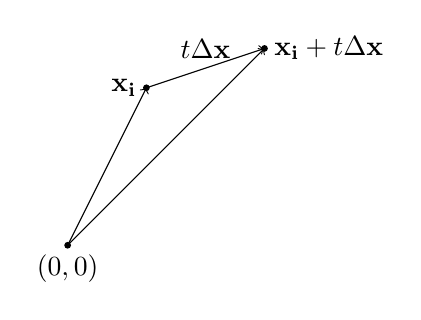
\begin{tikzpicture}
		\filldraw (0, 0) circle (1pt) node[below]{$(0, 0)$};
		\filldraw (1, 2) circle (1pt) node[left]{$\mathbf{x_{i}}$};
		\filldraw (2.5, 2.5) circle (1pt) node[right]{$\mathbf{x_{i}} + t \Delta \mathbf{x}$};
		\draw[->] (0, 0) -- (1, 2);
		\draw[->] (1, 2) -- node[pos=0.5, above]{$t \Delta \mathbf{x}$} (2.5, 2.5);
		\draw[->] (0, 0) -- (2.5, 2.5);
	\end{tikzpicture}
\end{figure}  
Now consider $f(\mathbf{x})$ is convex. According to the first-order condition, we have:
\begin{equation*}
	f(\mathbf{x_{i} + t \Delta \mathbf{x}}) \geq f(\mathbf{x_{i}}) + \nabla f(\mathbf{x_{i}})^{T} (t \Delta \mathbf{x_{i}})
\end{equation*}
We notice from this inequality that if $ \nabla f(\mathbf{x_{i}})^{T} (t \Delta \mathbf{x_{i}}) \geq 0$, $f(\mathbf{x_{i} + t \Delta \mathbf{x}}) \geq f(\mathbf{x_{i}})$ always holds. Hence, we must choose $t$ and $\Delta \mathbf{x}$ that satisfied:
\begin{equation*}
	\nabla f(\mathbf{x_{i}})^{T} t \Delta \mathbf{x} \leq 0
\end{equation*}
By considering $t > 0$, we notice the above inequality is equivalent to:
\begin{equation}
	\nabla f(\mathbf{x_{i}})^{T} \Delta \mathbf{x} \leq 0
	\label{descent}
\end{equation}
Which means, we must choose the incremental direction that is opposite of the gradient direction.

\subsection{Optimization under Approximation Perspective}
For a convex function $f(\mathbf{x})$, we can use Taylor Approximation to approximate any point $\mathbf{y}$ base on a fixed point $\mathbf{x}$ as:
\begin{equation}
		f(\mathbf{y}) = f(\mathbf{x}) + \nabla f(\mathbf{x})^{T} (\mathbf{y} - \mathbf{x}) + \frac{1}{2} (\mathbf{y} - \mathbf{x})^{T} \nabla^{2} f(\mathbf{z}) (\mathbf{y} - \mathbf{x})
		\label{appro}
\end{equation}
Where $\mathbf{z}$ could be any point within $\mathbf{dom} f$. If we further consider $f$ as a \textit{strong convex} function, which means, there exist some $\alpha$, so that the function $g(\mathbf{x})$:
\begin{quote}
	\center
	$g(\mathbf{x}) = f(\mathbf{x}) - \alpha \| \mathbf{x} \|^{2}_{2}$ is convex
\end{quote}
Since $g(\mathbf{x})$ is convex, we have:
\begin{equation*}
	\nabla^{2} g(\mathbf{x}) = \nabla^{2} f(\mathbf{x}) - \alpha \mathbf{I} \succeq 0
\end{equation*}
Which implicit that for any $\mathbf{z} \in \mathbf{dom} f$, there is:
\begin{equation*}
	\nabla^{2} f(\mathbf{z}) \succeq \alpha \mathbf{I}
\end{equation*}
We can apply this inequality to Equation \ref{appro} and hence:
\begin{equation}
	\begin{aligned}
		f(\mathbf{y}) &= f(\mathbf{x}) + \nabla f(\mathbf{x})^{T} (\mathbf{y} - \mathbf{x}) + \frac{1}{2} (\mathbf{y} - \mathbf{x})^{T} \nabla^{2} f(\mathbf{z}) (\mathbf{y} - \mathbf{x}) \\
		&\geq f(\mathbf{x}) + \nabla f(\mathbf{x})^{T} (\mathbf{y} - \mathbf{x}) + \frac{1}{2} (\mathbf{y} - \mathbf{x})^{T} \alpha \mathbf{I} (\mathbf{y} - \mathbf{x}) \\
		&= f(\mathbf{x}) + \nabla f(\mathbf{x})^{T} (\mathbf{y} - \mathbf{x}) + \frac{\alpha}{2} \| \mathbf{y} - \mathbf{x} \|^{2}_{2}
	\end{aligned}
	\label{bound}
\end{equation}
Therefore, we successfully construct a lower bound of any point $\mathbf{y}$ in terms of a fix point $\mathbf{x}$. Now, we can substitute $\mathbf{y}$ by $\mathbf{x_{i + 1}}$ and fix $\mathbf{x}$ as $\mathbf{x_{i}}$. In order to make $f(\mathbf{x_{i + 1}}) \leq f(\mathbf{x_{i}})$, we need to choose a point $\mathbf{x_{i + 1}}$ that can minimize $f(\mathbf{x_{i + 1}})$. Indeed, we can choose the lower bound in Equation \ref{bound} as the approximation of $f(\mathbf{x_{i + 1}}) \approx f(\mathbf{x_{i}}) + \nabla f(\mathbf{x_{i}})^{T} (\mathbf{x_{i + 1}} - \mathbf{x_{i}}) + \frac{\alpha}{2} \| \mathbf{x_{i + 1}} - \mathbf{x_{i}} \|^{2}_{2}$ (Since we can think $\mathbf{x_{i}}$ as constant, the term $f(\mathbf{x_{i}})$ is also a constant) and then, minimize this approximation instead of minimizing the original $f(\mathbf{x_{i + 1}})$ and construct a simple minimization problem:
\begin{equation*}
	\displaystyle\min_{\mathbf{x_{i + 1}}} \quad f(\mathbf{x_{i}}) + \nabla f(\mathbf{x_{i}})^{T} (\mathbf{x_{i + 1}} - \mathbf{x_{i}}) + \frac{\alpha}{2} \| \mathbf{x_{i + 1}} - \mathbf{x_{i}} \|^{2}_{2}
\end{equation*}
The solution of this optimization is:
\begin{equation*}
	\mathbf{x_{i + 1}} = \mathbf{x_{i}} - \frac{1}{\alpha} \nabla f(\mathbf{x_{i}})
\end{equation*}
Which is equivalent to Equation \ref{iter} by setting $t = \frac{1}{\alpha}$ and $\Delta \mathbf{x} = - \nabla f(\mathbf{x_{i}})$. Indeed, we can verify that by letting $\Delta \mathbf{x} = - \nabla f(\mathbf{x_{i}})$, Equation \ref{descent} always holds as: 
\begin{equation*}
	\begin{aligned}
		\nabla f(\mathbf{x_{i}})^{T} \Delta \mathbf{x} &= - \nabla f(\mathbf{x_{i}})^{T} \nabla f(\mathbf{x_{i}}) \\
		&= - \| \nabla f(\mathbf{x_{i}}) \|^{2}_{2} \\
		&\leq 0
	\end{aligned}
\end{equation*}
In fact, the optimization method which choosing $- \nabla f(\mathbf{x_{i}})$ as incremental direction is called \textit{Gradient Descend}.

\subsection{Gradient Descend and Line Search}
As we discussed before, by letting $\Delta \mathbf{x} = -\nabla f(\mathbf{x_{i}})$ in Equation \ref{iter}, we get the Gradient Descend Method. After we have chosen the incremental direction, one more thing we need to concern is the value of $t$, or be more specific, the incremental length. We first notice that within the first-order condition:
\begin{equation*}
	f(\mathbf{x_{i}} + t \Delta \mathbf{x}) \geq f(\mathbf{x_{i}}) + t \nabla f(\mathbf{x_{i}})^{T} \Delta \mathbf{x_{i}}
\end{equation*} 
If we force $t$ to be large, the term $t \nabla f(\mathbf{x_{i}})^{T} \Delta \mathbf{x_{i}}$ could be very negative. As a result, the first-order condition can still hold even though $f(\mathbf{x_{i}}) \geq f(\mathbf{x_{i}} + t \Delta \mathbf{x})$, which against our intention: $f(\mathbf{x_{i}}) \leq f(\mathbf{x_{i}} + t \Delta \mathbf{x})$. On the other hand, if we choose $t$ to be too small, the term $\mathbf{x_{i}} + t \Delta \mathbf{x}$ is almost identical to original $\mathbf{x_{i}}$, which means, the algorithm converge very slowly. The process that find the value of $t$ is called \textit{line search}. One general idea for addressing line search is that we can first assign $t$ with an initial value, \textsl{e.g.} $t_{init} = 1$, then reduce the value of $t$ iterative until it satisfied some constrain. This idea left us with 2 question:
	\begin{enumerate}
		\item what is the stop constrain
		\item what is the decrease size of $t$ in each iteration
	\end{enumerate}
For the first question, we first notice that we can approximate $f(\mathbf{x_{i}} + t \Delta \mathbf{x})$ by using first order Taylor Approximation:
\begin{equation*}
	f(\mathbf{x_{i}} + t \Delta \mathbf{x}) \approx f(\mathbf{x_{i}}) + t \nabla f(\mathbf{x_{i}})^{T} \Delta \mathbf{x}
\end{equation*}
The above equation hold when $t$ is very small. Since $\Delta \mathbf{x} = - \nabla f(\mathbf{x_{i}})$, we can multiple the term $t \nabla f(\mathbf{x_{i}})^{T} \Delta \mathbf{x}$ with an $\alpha < 1$ and get:
\begin{equation*}
	f(\mathbf{x_{i}}) + t \nabla f(\mathbf{x_{i}})^{T} \Delta \mathbf{x} \leq f(\mathbf{x_{i}}) + t \alpha \nabla f(\mathbf{x_{i}})^{T} \Delta \mathbf{x}
\end{equation*}
Combine these two equations, we can conclude that for any $0 < \alpha < 1$, there exist a small enough $t$ that satisfied:
\begin{equation}
	f(\mathbf{x_{i}} + t \Delta \mathbf{x}) \leq f(\mathbf{x_{i}}) + t \alpha \nabla f(\mathbf{x_{i}})^{T} \Delta \mathbf{x}
	\label{backtrack}
\end{equation}
Indeed, Equation \ref{backtrack} give us a good stopping constrain for line search, we can select an $\alpha$ and reduce the value of $t$ iterative until this equation is satisfied. For the second question, we can reduce $t$ by multiplying it with a $\beta$ which satisfied $0 < \beta < 1$.

This line search algorithm is called \textit{backtrack line search} and can be summarized as:
\begin{enumerate}
	\item Choose the value of $\alpha$ and $\beta$
	\item Choose the initial value of $t$
	\item Multiple $t$ with $\beta$ and assign $t$ with this new value($t := \beta t$) until Equation \ref{backtrack} is satisfied.
	\item Return the value of $t$.
\end{enumerate}

\subsection{Newton's Method}
According to the above discussion, we have noticed that we can minimize $f(\mathbf{x} + \Delta \mathbf{x})$ by minimize it's approximation. Particularly, by minimizing the first-order Taylor Approximation of $f(\mathbf{x} + \Delta \mathbf{x})$, we obtain Gradient Descent algorithm. Indeed, instead of using first-order approximation, we can use second-order Taylor Approximation of $f(\mathbf{x} + \Delta \mathbf{x})$. Thus, we have:
\begin{equation*}
	f(\mathbf{x} + \Delta \mathbf{x}) \approx f(\mathbf{x}) + \nabla f(\mathbf{x})^{T} \Delta \mathbf{x} + \frac{1}{2} \Delta \mathbf{x}^{T} \nabla^{2} f(\mathbf{x}) \Delta \mathbf{x}
\end{equation*}
By minimizing this approximation over $\Delta \mathbf{x}$(in here, $\mathbf{x}$ is the initial point we choose hence, is a constant), we have:
\begin{equation*}
	\Delta \mathbf{x} = -\nabla^{2} f(\mathbf{x})^{-1} \nabla f(\mathbf{x})
\end{equation*}

\subsection{Steepest Descent}
The Gradient Descent Algorithm we introduced before is a special case of a more general algorithm called \textit{Steepest Descent}. As we discussed before, for a initial point $\mathbf{x}$, we want to find an incremental direction $\Delta \mathbf{x}$ and a incremental size $t$ so that: $f(\mathbf{x} + t \Delta \mathbf{x}) \leq f(\mathbf{x})$. Be more specific, we want to minimize $f(\mathbf{x} + t \Delta \mathbf{x})$. In order to do so, we can minimize the approximation of $f(\mathbf{x} + t \Delta \mathbf{x})$ instead of the original function. Moreover, according to the first-order Taylor Approximation, we have:
\begin{equation*}
	f(\mathbf{x} + t \Delta \mathbf{x}) \approx f(\mathbf{x}) + \nabla f(\mathbf{x})^{T} t \Delta \mathbf{x}
\end{equation*}
Since $\mathbf{x}$ is an initial point and $t$ is the incremental size that can be found through line search, we can treat these $\mathbf{x}$ and $t$ as constant. Therefore, in order to minimize the approximation function, we only need to minimize the term $\nabla f(\mathbf{x}) \Delta \mathbf{x}$ (as we have treated $f(\mathbf{x})$ and $t$ as constants). As a result, we can find $\Delta \mathbf{x}$ by solving following equation:
\begin{equation*}
	\Delta \mathbf{x} = \argmin_{\Delta \mathbf{x}} \nabla f(\mathbf{x})^{T} \Delta \mathbf{x}
\end{equation*}
We then notice that $\nabla f(\mathbf{x})^{T} \Delta \mathbf{x}$ is a affine(linear) function, which means, it can reach $-\infty$ if $\Delta$ is unconstrained. Additionally, the first-order Taylor Approximation only hold when $t \Delta \mathbf{x}$ is small enough, therefore, if $\Delta \mathbf{x}$ is unconstrained and being too large, we cannot use $f(\mathbf{x}) + \nabla f(\mathbf{x})^{T} t \Delta \mathbf{x}$ to approximate the original function and hence, the minimization of $f(\mathbf{x}) + \nabla f(\mathbf{x})^{T} t \Delta \mathbf{x}$ is useless under this situation. As a result, it is important to add some constrain over $\Delta \mathbf{x}$. The common constrain is restricting the norm of $\Delta \mathbf{x}$. Therefore, we can find $\Delta \mathbf{x}$ by solving the following optimization problem:
\begin{equation*}
	\begin{aligned}
		\displaystyle\min_{\Delta \mathbf{x}} \quad & \nabla f(\mathbf{x})^{T} \Delta \mathbf{x} \\
		\textsl{s.t.} \quad & \| \Delta \mathbf{x} \| \leq 1
	\end{aligned}
\end{equation*}
The $\| \Delta \mathbf{x} \|$ could mean any order norm, \textsl{e.g.} first order norm $\| \Delta \mathbf{x} \|_{1}$, second order norm $\| \Delta \mathbf{x} \|_2$.
\section{Optimization Algorithm with Inequality Constrain}
The inequality constrains within optimization problem are usually the most difficulty part to deal with. Therefore, finding a method to eliminate these constrain within optimization problems will help solve these problems. Indeed, for an optimization problem:
\begin{equation*}
	\begin{aligned}
		\displaystyle\min_{\mathbf{x}} \quad & f_{0}(\mathbf{x}) \\
		\textsl{s.t.} \quad & f_{i}(\mathbf{x}) \leq 0 \quad i = 1, 2, \cdots, n \\
		& h_{j}(\mathbf{x}) = 0 \quad j = 1, 2, \cdots, m
	\end{aligned}
\end{equation*}
We can think the inequality constrain serve the following purpose: The inequality constrains define a set of $\mathbf{x}$, if $\mathbf{x}$ take value out of this set, the objective function($f_{0}(\mathbf{x})$) will take value $\infty$. Therefore, we can embed the inequality constrains into objective function by replacing them with the \textit{indicator function} defined as:
\begin{equation*}
	\mathcal{I}(u) = 
	\begin{cases}
		0 \quad u \leq 0\\
		\infty \quad u > 0
	\end{cases}
\end{equation*} 
Being more specific, we can reconstruct the optimization problem with indicator function as:
\begin{equation*}
	\begin{aligned}
		\displaystyle\min_{\mathbf{x}} \quad & f_{0}(\mathbf{x}) + \displaystyle\sum_{i = 1}^{n} \mathcal{I}(f_{i}(\mathbf{x})) \\
		\textsl{s.t.} \quad & h_{j}(\mathbf{x}) = 0 \quad j = 1, 2, \cdots, m
	\end{aligned}
\end{equation*}
Following the definition of indicator function, it can be seen that the new objective function $f_{0}(\mathbf{x}) + \displaystyle\sum_{i = 1}^{n} \mathcal{I}(f_{i}(\mathbf{x}))$ will goes to infinity if $f_{i}(\mathbf{x}) \leq 0$ is not satisfied and will equal to the original objective function $f_{0}(\mathbf{x})$ if the inequality constrains are hold.

Even though we successfully remove the inequality constrains, it is still difficulty to deal with the indicator function as it is non differentiable. A better idea is using some approximation function to replace indicator function. Particularly, a good approximation function $\phi(u)$ need to have the similar property as indicator function: $\phi(u)$ will approximate 0 if $u \leq 0$ and approximate $\infty$ if $u > 0$. One such function is \textit{log-barrier} function defined as:
\begin{equation*}
	\phi(u) = -\frac{1}{t}\log{(-u)}
\end{equation*}
Where $t$ is a constant chosen by us. By applying this approximation to the original problem, we have:
\begin{equation*}
	\begin{aligned}
		\displaystyle\min_{\mathbf{x}} \quad & f_{0}(\mathbf{x}) + \frac{1}{t} \displaystyle\sum_{i = 1}^{n} -\log{(- f_{i}(\mathbf{x}))} \\
		\textsl{s.t.} \quad & h_{j}(\mathbf{x}) = 0 \quad j = 1, 2, \cdots, m
	\end{aligned}
\end{equation*}
For our convenience, we can defined:
\begin{equation*}
	\Phi(\mathbf{x}) = \displaystyle\sum_{i = 1}^{n} -\log{(- f_{i}(\mathbf{x}))}
\end{equation*}
Recalling the equivalent problem construction methodology, we can construct a equivalent problem by multiplying the original objective function with any constant since this action will not effect the optimal point. Therefore, we can construct an equivalent problem by multiplying the objective function in above optimization problem with constant $t$ and get:
\begin{equation*}
	\begin{aligned}
		\displaystyle\min_{\mathbf{x}} \quad & t f_{0}(\mathbf{x}) + \Phi(\mathbf{x}) \\
		\textsl{s.t.} \quad & h_{j}(\mathbf{x}) = 0 \quad j = 1, 2, \cdots, m
	\end{aligned}
\end{equation*} 
As a result, we can solve the original optimization by solving this approximation problem. Now, let us have a closer look of log-barrier method by considering the stand form convex optimization problem. Following our discussion above, we can construct the approximation problem as:
\begin{equation*}
	\begin{aligned}
		\displaystyle\min_{\mathbf{x}} \quad & t f_{0}(\mathbf{x}) + \Phi(\mathbf{x}) \\
		\textsl{s.t.} \quad & \mathcal{A}\mathbf{x} = \mathbf{b}
	\end{aligned}
\end{equation*} 
The first step to solve this problem is constructing its Lagrangian:
\begin{equation*}
	\mathcal{L}(\mathbf{x}, \nu) = t f_{0}(\mathbf{x}) + \Phi(\mathbf{x}) + \nu^{T}(\mathcal{A} \mathbf{x} - \mathbf{b})
\end{equation*}
Now, suppose this problem has optimal point $\mathbf{x^{*}}$. This optimal point must be the minimizer of Lagrangian, which means, there must exist a $\nu^{*}$ so that:
\begin{equation*}
	\nabla \mathcal{L}(\mathbf{x}^{*}, \nu^{*}) = 0
\end{equation*}
By noticing that
\begin{equation*}
	\nabla \Phi(\mathbf{x}) = \displaystyle\sum_{i = 1}^{n} \frac{1}{-f_{i}(\mathbf{x})} \nabla f_{i}(\mathbf{x})
\end{equation*}
We have:
\begin{equation}
	\begin{aligned}
		\nabla \mathcal{L}(\mathbf{x}^{*}, \nu^{*}) & = t \nabla f_{0}(\mathbf{x^{*}}) + \displaystyle\sum_{i = 1}^{n} \frac{1}{-f_{i}(\mathbf{x^{*}})} \nabla f_{i}(\mathbf{x^{*}}) + \mathcal{A}^{T} \nu \\
		& = 0
	\end{aligned}
	\label{equ}
\end{equation}
This equation indicates that the approximation problem has optimal solution if and if this equation hold. Indeed, we can multiple Equation \ref{equ} with $\frac{1}{t}$ and get:
\begin{equation*}
	\nabla f_{0}(\mathbf{x^{*}}) + \displaystyle\sum_{i = 1}^{n} \frac{1}{-t f_{i}(\mathbf{x^{*}})} \nabla f_{i}(\mathbf{x^{*}}) + \mathcal{A}^{T} \frac{\nu}{t} = 0
\end{equation*}
It is not hard to find out that the term $\nabla f_{0}(\mathbf{x^{*}}) + \displaystyle\sum_{i = 1}^{n} \frac{1}{-t f_{i}(\mathbf{x^{*}})} \nabla f_{i}(\mathbf{x^{*}}) + \mathcal{A}^{T} \frac{\nu}{t}$ is the first-order derivative of the Lagrangian $\hat{\mathcal{L}}(\mathbf{x}, \hat{\lambda}, \hat{\nu})$ of the original optimization problem with $\hat{\lambda}_{i} = \frac{1}{-tf_{i}(\mathbf{x})}$ and $\hat{\nu} = \frac{\nu}{t}$. As a result, the Equation \ref{equ} also indicates $\mathbf{x^{*}}$ minimize $\hat{\mathcal{L}}(\mathbf{x},  \hat{\lambda}, \hat{\nu})$ and hence, the Lagrange Dual Function of original optimization function can be obtained as:
\begin{equation*}
	g(\hat{\lambda}, \hat{\nu}) = f_{0}(\mathbf{x^{*}}) + \displaystyle\sum_{i = 1}^{n} \hat{\lambda}_{i} f_{i}(\mathbf{x^{*}}) + \hat{\nu}^{T} (\mathcal{A} \mathbf{x}^{*} - \mathbf{b})
\end{equation*}
By substituting $\hat{\lambda}_{i} =  \frac{1}{-tf_{i}(\mathbf{x}^{*})}$ to this equation and notice $\mathcal{A} \mathbf{x}^{*} - \mathbf{b} = 0$, we have:
\begin{equation*}
	g(\hat{\lambda}, \hat{\nu}) = f_{0}(\mathbf{x^{*}}) - \frac{n}{t}
\end{equation*}
Where $n$ is the number of inequality constrains. One important thing to note here is that the pair $(\hat{\lambda}, \hat{\nu})$ do not maximize the Lagrange Dual Function, therefore, we have:
\begin{equation*}
	p^{*} \geq g(\hat{\lambda}, \hat{\nu}) = f_{0}(\mathbf{x^{*}}) - \frac{n}{t}
\end{equation*}
Where $p^{*}$ is the optimal value of the original problem. As a result, we have:
\begin{equation*}
	f_{0}(\mathbf{x^{*}}) - p^{*} \leq \frac{n}{t}
\end{equation*}
Which measure the margin between the optimal value of approximation problem $f(\mathbf{x}^{*})$ and the optimal value of original problem $p^{*}$.
\section{Application}

\end{document}
